\section{An example : The Double Integrator}
Consider a double integrator system with unit mass in two dimension : 
\begin{equation}
    \ddot{\qv} = \uv
\end{equation}
where $\qv \in \mathbb{R}^2$ represents the planar position of the robot and $\uv \in \mathbb{R}^2$, the torque commands.
%A possible unsafe tracking controller which allows the robot to go from $\qv_{start}$ to $\qv_{goal}$ without taking into account the obstacles is given by :
We are going to solve the problem of navigating the system from $\qv_{start}$ to $\qv_{goal}$ while avoiding obstacles, firstly,  in a model-free fashion and, then, in the classical full-model based approach.
We work with multiple obstacles with  different radii but  there will be considered  the closest one at each time.\\ \\
\textbf{Model-free Approach}:
A solution which allows to navigate the system from $\qv_{start}$ to $\qv_{goal}$ without taking into account the obstacles consists in realizing the desired velocity $\dot{\qv}_{goal}$:   
\begin{equation}
    \dot{\qv}_{goal}=-K_p(\qv - \qv_{goal}),\,K_p\in\mathbb{R}_{>0}
\end{equation}
 We can avoid an obstacle of radius $R$ centered at $\qv_O$ by defining $d = \lVert \qv-\qv_O \rVert$ and the CBF:
\begin{equation}
h(\qv)=d-R
\end{equation}
with gradient $\nabla h(\qv) = \frac{\qv-\qv_O}{d} = \nv_0^T$ with the unit vector $\nv_0$ pointing from the obstacle to the robot. Then, we modify $\dot{\qv}_{goal}$ in a minimally invasive fashion by solving the quadratic optimization program:
\begin{align}
    &\argmin_{\dot{\qv}_{safe} \in \mathbb{R}^2} \,\,(\dot{\qv}_{safe}-\dot{\qv}_{goal})^T(\dot{\qv}_{safe}-\dot{\qv}_{goal}) \notag\\
    &\mathrm{s.t} \,\,\, \nv_0^T \dot{\qv}_{safe}\geq -\alpha(d-R)
\end{align}
Then, by defining $\xv = \dot{\qv}, \xv_{safe}=\dot{\qv}_{safe}$, the safe velocity tracking controller $\uv = K_d (\xv - \xv_{goal}), K_d \in \mathbb{R}_{>0} $ guarantees the asynptotic convergence of $\xv$ to $\xv_{safe}$. \\
\textbf{Remark 1.} The double integrator system avoids the obstacles, although the second-order dynamics was not directly taken into account during the CBF and control design. It follows that the CBF has relative degree $1$ with respect to $y = \qv$ if we are assuming to control the robot in velocities i.e. $\dot{\qv}=\vv$. \\
\textbf{Remark 2.} The condition for safety consists in picking a small enough $\alpha$-value (e.g $0.1$,$0.2$).

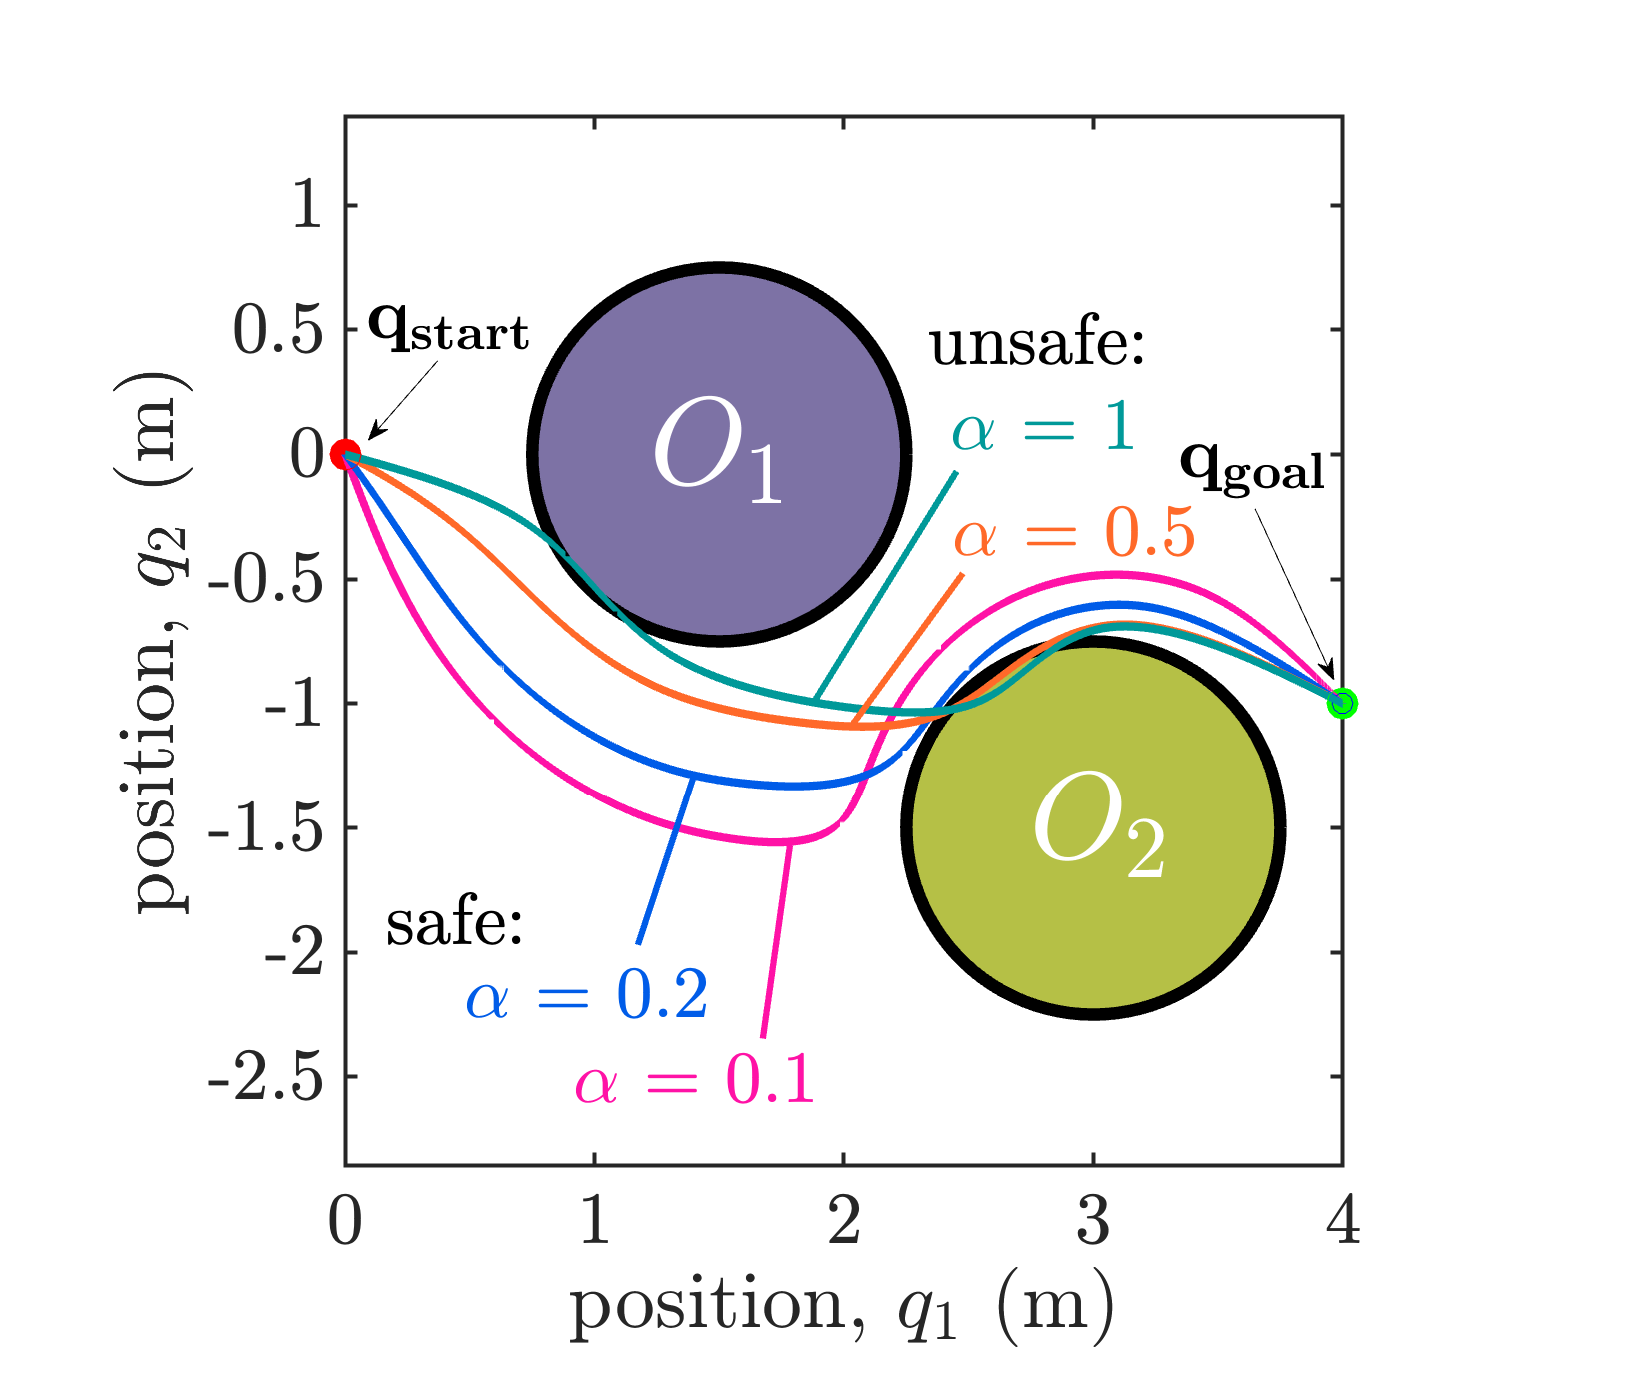
\includegraphics[scale=0.65]{figprint.eps}\\
